\chapter{Perspectiva de Solução} \label{chap:solução}

O reconhecimento facial em imagens sofreu uma evolução notável nos últimos 20 anos, tal como documentado no capítulo \ref{chap:reco} deste relatório. 

Em cenários cooperativos com condições de captura de imagens controladas, nomeadamente ao nível da pose, iluminação e expressões faciais, considera-se mesmo que o problema de verificação 1:1 se encontra resolvido, uma vez que as taxas de reconhecimento atingidas são satisfatórias para a grande maioria das aplicações \citep{Li2011}. Existem também várias aplicações em situações reais com um bom nível de satisfação por parte dos seus utilizadores, como é o caso do sistema de fronteira automático dos aeroportos portugueses, ou o controlo de entradas nas cerimónias inaugurais dos jogos olímpicos de Pequim. Em condições favoráveis, é então possível considerar que os sistemas de reconhecimento facial automático atuais conseguem mesmo ultrapassar a capacidade de reconhecimento humana, uma vez que conseguem identificar com precisão um maior número de faces do que aquelas que um humano consegue.

Contudo, o problema de reconhecimento facial automático ainda se encontra longe de ser um problema totalmente resolvido. Em cenários onde é registada uma grande variação ao nível da pose, iluminação ou outros fatores identificados na secção \ref{desafios} deste relatório, a identificação das entidades capturadas é ainda uma tarefa desafiante  \citep{Li2011}. Para além disso, a performance e satisfação obtida por parte dos utilizadores dos sistemas atuais demonstra uma grande variação tendo em conta as situações onde estes sistemas são utilizados. 

Finalmente, a crescente ubiquidade tecnológica e poder computacional presente nos diversos dispositivos utilizados no nosso dia a dia, aumenta o leque de aplicações possíveis do reconhecimento facial automático, apresentando novos desafios às soluções de atualmente existentes.

Assim sendo, torna-se pertinente a continuação da investigação na área do reconhecimento facial em imagens. Para além disso, o elevado valor comercial das soluções existentes e consequente falta soluções abertas permite aos resultados alcançar uma grande visibilidade dos resultados obtidos.

Ao nível da abstração de imagens, estudos efetuados demonstraram que aplicação destes filtros na recuperação de informação multimédia, nomeadamente no âmbito da da ilustração automática de texto têm a potencialidade de melhorar a informação retornada, assim como reduzir significativamente as necessidades de processamento e armazenamento \citep{Coelho2012}. 

Tendo a importância da investigação na área do reconhecimento facial, e uma vez que não existem estudos relativos à utilização de filtros de abstração no processo de reconhecimento facial, torna-se pertinente o estudo do seu impacto.

A hipótese levantada no âmbito desta dissertação é então que o uso de a abstração em imagens que vão ser ser alvo de reconhecimento facial pode melhorar a qualidade do reconhecimento.

\section{Objetivos} \label{sec:objetivosperpectiva}
O principal objetivo deste projeto visa o estudo do impacto de filtros de abstração visual de informação no processo de reconhecimento facial automático em imagens. Para isso, destacam-se o seguinte conjunto de objetivos parciais:

\begin{enumerate}
\item Desenvolvimento de um sistema de reconhecimento facial de personalidades;
\item Integração da abstração de imagens no sistema desenvolvido;
\item Avaliação dos resultados da abstração de imagens no processo de reconhecimento facial;
\end{enumerate}

Da avaliação efetuada, para além da publicação desta dissertação, espera-se ainda a publicação de um artigo científico onde sejam descritos os resultados obtidos.

\section{Implementação} \label{sec:implementacao}

Uma vez que não se pretende no âmbito desta dissertação efetuar investigação ao nível dos algoritmos de reconhecimento facial, mas sim ao nível do impacto do uso de imagens abstraídas nesse sistemas, a implementação desses algoritmos terá por base a utilização de soluções abertas de reconhecimento facial, nomeadamente a biblioteca \textit{Open CV (Open Source Computer Vision)}.

Ao nível dos filtros de abstração o estudo será efetuado utilizado o filtro \textit{Anisotropic Kuwahara}.
Este filtro foi utilizado anteriormente, e com resultados positivos, em abstração de imagens para a recuperação de informação multimédia, pelo que se considera adequada a sua utilização no âmbito deste projeto.

Por último, ao nível da coleção de dados a analisar, e uma vez que este projeto se encontra a ser desenvolvido em parceria com o laboratório da Sapo da FEUP, temos em vista analisar a coleção de imagens Sapo Fama, a qual agrega uma base de dados de imagens de personalidades famosas nacionais e internacionais.
	
\subsection{OpenCV - Face Recognizer}
O \textit{OpenCV} é uma biblioteca de código aberto nas áreas de visão por computador e \textit{machine learning}, onde se encontra disponível a implementação de mais de 2500 algoritmos. Esta biblioteca possui uma comunidade de mais de 47 mil pessoas, já registou mais de 5 milhões de downloads e é utilizada globalmente por empresas como a Google, Yahoo, Microsoft, Intel, IBM, Sony, Honda, Toyota \cite{Team}. 

Ao nível do reconhecimento facial, esta biblioteca disponibiliza um módulo denominado \textit{Face Recognizer}, onde se encontra implementados os algoritmos \textit{Eigenfaces}, \textit{Fisherfaces} e \textit{Local Binary Patterns Histograms}.

Tendo em conta a ampla utilização da biblioteca OpenCV e a sua constante atualização pela sua comunidade, assim como as facilidades providenciadas pelo módulo de reconhecimento facial, esta foi considerada a biblioteca ideal para utilizar como base de implementação do sistema de reconhecimento facial a criar. De seguida encontram-se brevemente descritos os três algoritmos implementados no módulo \textit{Face Recognizer:}

\subsubsection{Eigenfaces}
O método \textit{Eigenfaces} foi introduzido por \cite{Belhumeur1997} e tira partido da Análise dos Componentes Principais (ACP) para efetuar o reconhecimento facial automático.

A análise de componentes principais tem como objetivo determinar as relações existentes entre diferentes conjuntos de dados, nomeadamente ao nível das suas diferenças e semelhanças, tirando partido da redundância existente para criar uma representação reduzida dos dados sem que a perda de informação ocorrida seja significativa. As imagens faciais possuem uma grande redundância natural, o algoritmo \textit{Eigenfaces}, através da análise dos componentes principais dessas imagens, efetua uma projeção das imagens faciais num sub-espaço onde se evidenciam apenas as variações entre as diversas caras conhecidas pelo sistema.

A redução do espaço de representação revela-se fulcral no problema de reconhecimento facial em imagens, devido à grande dimensionalidade exigida para a representação de uma face, considerando, por exemplo, uma dada imagem de $nxm$ \textit{pixels} de tons cinzentos, essa imagem poderia ser traduzida por um espaço vetorial de $m = nxm$ \textit{pixels}, assim sendo, uma imagem de apenas $200x200$ \textit{pixels} necessitaria de um total de $400000$ \textit{pixels} para ser representada.

O processo de reconhecimento facial com recurso ao algoritmo \textit{Eigenfaces} consiste então nos seguintes passos:
\begin{enumerate}
\item Aquisição de um conjunto de dados iniciais (conjunto de treino);
\item Projeção dos dados obtidos num sub-espaço de faces através da ACP;
\item Aquisição de uma imagem a reconhecer;
\item Projeção da face a reconhecer no sub-espaço do conjunto de treino, calculando as distâncias obtidas para cada face conhecida pelo sistema;
\item Determinar qual o face do conjunto de treino com menor distância à face a reconhecer;
\item Caso a distância para a face obtida seja menor do que um limite operacional estabelecido, a imagem é reconhecida como sendo essa pessoa, caso contrário, a face é identificada como sendo uma pessoa desconhecida pelo sistema.
\end{enumerate}

Este método efetua assim uma abordagem holística ao problema de reconhecimento facial em imagens, uma vez que tem em consideração a representação facial como um todo, não fazendo a distinção entre pontos específicos da face como olhos, orelhas ou nariz para efetuar o reconhecimento facial. Uma vantagem deste tipo de representação é a reduzida sensibilidade ao ruído presente nas imagens \cite{Zhao2003}.

\subsubsection{Fisherfaces}
A análise dos componentes principais visa determinar o sub-espaço onde se verifica uma maior variação entre um conjunto de imagens, no entanto, a variação na representação facial de uma pessoa encontra-se muitas vezes relacionada com mudanças de expressões faciais ou iluminação dos indivíduos. Assim sendo, o sub-espaço criado pelo algoritmo \textit{Eigenfaces} não traduz muitas vezes as apenas as diferenças de identidade entre os diversos indivíduos, mas também as diferenças verificadas ao nível das condições de captura das imagens, mesmo considerando o mesmo indivíduo devido à sua tolerância reduzida em termos de representação das variações intra-indivíduo. O algoritmo \textit{Fisherfaces} tenta resolver este problema, através da aplicação de um passo de \textit{Linear Discriminant Analysis (LDA)} após a análise dos componentes principais, de forma a determinar mais corretamente as variações intra-classe existentes no conjunto de imagens a avaliar.

A LDA tenta maximizar as diferenças existentes entre diferentes indivíduos(inter-classe) e minimizar as variações entre imagens da mesma pessoa(intra-classe) de modo a obter uma representação mais robusta em termos de variação ao nível da iluminação.






\subsubsection{Local Binary Patterns Histograms}
lorem ipsum

\subsection{Filtro \textit{Anisotropic Kuwahara}}
\begin{figure}[h]
  \begin{center}
    \leavevmode
    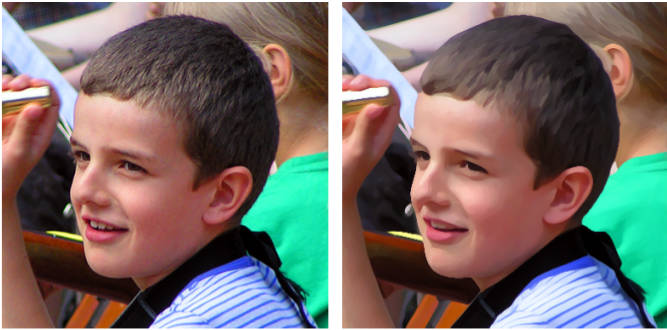
\includegraphics[width=0.7\textwidth]{filterskid}
    \caption{Comparação entre imagem não abstraída (esquerda) e imagem abstraída (direita).}	
    \label{fig:filterskid}
  \end{center}
\end{figure}

Ao nível dos filtros de abstração o estudo será efectuado utilizado o filtro Anisotropic Kuwahara (FAK).

Este filtro consiste numa generalização do filtro Kuwahara que remove alguns artefactos originados na aplicação do filtro original através da adaptação da forma, escala e orientação do filtro à estrutura local das características da imagem \cite{Kyprianidis2009}. Desta forma é produzido um efeito de abstração tipo pintura, onde é removida informação não essencial em zonas de elevado contraste, enquanto são preservados os limites representados nas zonas de menor contraste, tal como demonstrado na figura \ref{fig:filterskid}. As imagens ficam assim com a clareza de uma ilustração, mas preservam a informação direcional tal como nas pinturas a óleo clássicas. Por outro lado, este filtro tira partido da placa gráfica para a realização da abstração das imagens, tornando-se assim particularmente indicado para o processamento de um elevado número de fotografias.

O filtro em questão foi também utilizado anteriormente, e com resultados positivos, em abstração de imagens para a recuperação de informação multimédia. 

Tendo em conta os fatores apresentados consideramos que este filtro é o mais adequado para a utilização no âmbito deste projeto.

\subsection{Coleções de dados}
Ao nível das coleções de dados a analisar serão utilizadas duas coleções de dados Sapo Fama e \textit{Labeled Faces in the Wild}.

\subsubsection{Sapo Fama}
A coleção Sapo Fama será obtida no âmbito da integração desta dissertação no laboratório da Sapo da Universidade do Porto. Este galeria multimédia agrega uma coleção de imagens utilizadas na plataforma online de notícias sobre personalidades públicas da Sapo e respetivas descrições textuais. As imagens contidas nesta coleção representam uma oportunidade única de avaliação do sistema desenvolvido numa biblioteca de imagens real e com elevado valor comercial. Na figura \ref{SapoFama} encontram-se representados alguns exemplos das imagens contidas nesta coleção. 

\begin{figure}[t]
  \begin{center}
    \leavevmode
    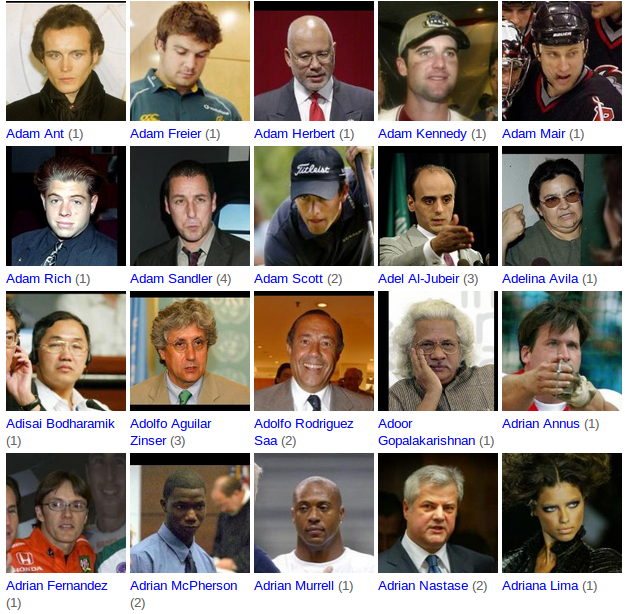
\includegraphics[width=1\textwidth]{lfw}
    \caption{Exemplos de imagens e respetivas anotações incluídas na biblioteca LFW}	
    \label{fig:lfwimagem}
  \end{center}
\end{figure}

\subsubsection{\textit{Labeled Faces in the Wild}}
A coleção \textit{Labeled Faces in the Wild (LFW)} é uma base de dados fotográfica desenhada especificamente para o estudo do problema de reconhecimento facial, particularmente em situações onde as condições de captura das imagens não possuem restrições. Esta coleção possuí 13233 imagens, de 5749 pessoas diferentes, sendo que dessas pessoas 1680 possuem mais do que uma imagem na galeria. O uso desta galeria no âmbito desta dissertação permitirá efetuar uma análise dos resultados obtidos num conjunto de dados standard e já previamente analisado por outros investigadores, assim como agilizar os testes dos sistemas desenvolvidos uma vez que a coleção já se encontra preparada especificamente para o estudo do desempenho de sistemas de reconhecimento facial automático. Na figura \ref{lbw} encontram-se representados alguns exemplos das imagens contidas nesta coleção.

\section{Avaliação Performance}

$amostras$ $biometricas$ capturas de características de uma pessoa que permitem efetuar o seu reconhecimento, no caso do reconhecimento facial em imagens, é o conjunto de fotografias que permite reconhecer uma pessoa.

$prova$ amostra biométrica apresentada ao sistema para ser reconhecida.

Conjuntos de imagens:

$\mathscr{G}$ designado de galeria, contem amostras biométricas das pessoas conhecidas para o sistema.

$\mathscr{P}_\mathscr{G}$ conjunto de provas de pessoas conhecidas pelo sistema, mas que são diferentes das amostras biométricas presentes na galeria.

$\mathscr{P}_\mathscr{N}$ conjunto de provas de pessoas não presentes na galeria, designados de impostores.

Dada uma prova $p_j$ apresentada ao sistema, essa prova é então comparada com toda a cada amostra biométrica da galeria $g_i$, resultando dessa comparação o respetivo índice de similaridade (\textit{similarity score}), $s_{ij}$.

$s_{ij}$ é designado de $match$ $score$, caso $g_i$ e $p_j$ sejam amostras da mesma pessoa, caso não o sejam é designado de $nonmatch$ $score$.

A função $id()$ retorna a identidade de uma amostra biométrica, em que $id(p_j) = id(g^*)$, sendo $g^*$ a única correspondência de $p_j$ na galeria e $s_{*j}$ o respetivo índice de similaridade.

\subsection{Identificação}
Tal como referido no capítulo \ref{chap:reco} deste relatório, em sistemas de reconhecimento facial automático o problema de identificação consiste na determinação da identidade de uma amostra biométrica (prova) fornecida ao sistema.

Na identificação de uma dada prova são calculados os índices de similaridade para todas as amostras na galeria, e ordenados os seus resultados. Uma prova $p_j$ tem ranking $n$ se o seu índice de similaridade for o enésimo maior índice de similaridade. Caso haja empates nos índices de similaridade é necessário resolver esses empates para determinar o ranking de uma prova, havendo para isso três métodos: otimista, pessimista e média. No método otimista,uma prova é associada ao ranking mais alto possível, obtido pelo número de índices estritamente maiores do que $s_{*j}$ mais um ($|> s_{*j}| + 1$). Na abordagem pessimista, um prova é associada ao ranking mais baixo possível, sendo esse devolvido pelo número de índices maiores ou iguais a $s_{*j}$ mais um ($|\geqslant s_{*j}| + 1$). Na média, tal como o seu nome indica é efetuada uma média entre os valores obtidos pelos métodos pessimista e otimista, sendo esta a abordagem mais utilizada. 

A performance da identificação em sistemas de reconhecimento facial pode ser avaliada em taxa de deteção e identificação e taxa de falso-alarme.

 \begin{description}
 \item[Taxa de deteção e identificação $(T_{DI})$:] Percentagem de provas do conjunto $\mathscr{P}_\mathscr{G}$ que são corretamente  identificadas. Uma prova é corretamente identificada caso o índice de similaridade para o seu $match$ $score$ seja seja maior do que um limite operacional pré-definido $\tau$.

\begin{equation}
 T_{DI}(\tau, n) = \frac{|\{p_j:p_j \in \mathscr{P}_\mathscr{G}, rank(p_j) \leqslant n, s_{*j} \geqslant \tau\}|}{|\mathscr{P}_\mathscr{G}|}
\end{equation}
 
  \item[Taxa de falso-alarme $(T_{FA})$:] Percentagem de impostores identificados erradamente, ou seja, percentagem de pessoas do conjunto de provas $\mathscr{P}_\mathscr{N}$, identificadas como alguém presente na galeria $\mathscr{G}$.
  
\begin{equation}
 T_{FA}(\tau) = \frac{|\{p_j:p_j \in \mathscr{P}_\mathscr{N}, s_{ij} \geqslant \tau\}|}{|\mathscr{P}_\mathscr{N}|}
\end{equation}

\end{description}

Um sistema de reconhecimento facial ideal teria uma taxa de deteção e identificação de 1.0 e uma taxa de falso-alarme de 0.0.

A modificação do valor de $\tau$ irá ter influência direta nas percentagens de deteção e falsos-alarmes calculadas. Ao aumentar o limite operacional, ambas as taxas diminuem, não sendo por isso possível maximizar ambos os valores, havendo sempre um compromisso entre o aumento da taxa de deteção e identificação e o aumento do número de falsos-alarmes. Este compromisso é tradicionalmente representado num gráfico do tipo \textit{receiver operating characteristic} (ROC). Um exemplo de um ROC encontra-se representado na figura \ref{roc}, com um ranking constante de 1. 

Outra forma de representar a performance de sistemas de reconhecimento facial é em função do ranking das provas presentes na galeria e encontra-se representada na figura \ref{roc2}. Nesta figura, o eixo vertical representa a taxa de deteção e reconhecimento e o eixo horizontal o ranking numa escala logarítmica. Cada curva representa a performance do mesmo sistema com uma diferente taxa de falso-alarme.

\subsection{Verificação}

Em situações de verificação da identidade, para além de uma amostra biométrica ($prova$) é também fornecida ao sistema a identidade da pessoa que se pretende identificar. Cabe ao sistema determinar se a identidade e amostra fornecidas pertencem à mesma pessoa. O sistema compara então a prova à amostra biométrica  da pessoa a quem corresponde a identidade fornecida guardada na galeria, dessa comparação é gerado o índice de similaridade entre a prova fornecida e os dados já armazenados no sistema. O sistema aceita como verdadeira a identidade fornecida caso o índice de similaridade seja superior a um  limite operacional fornecido.

Em termos formais, a verificação pode ser avaliada pela taxa de verificação e taxa de falsa-aceitação, as quais podem ser descritas da seguinte forma:

\begin{description}
 \item[Taxa verificação $(T_{V})$:] Percentagem de provas do conjunto $\mathscr{P}_\mathscr{G}$ que são corretamente verificadas.

\begin{equation}
 T_{V}(\tau, n) = \frac{|\{p_j:p_j \in \mathscr{P}_\mathscr{G}, s_{ij} \geqslant \tau, id(g_i)=id(p_j)\}|}{|\mathscr{P}_\mathscr{G}|}
\end{equation}

  \item[Taxa de falsa-aceitação $(T_{FA})$:] Percentagem de impostores aceites erradamente, ou seja, percentagem de pessoas do conjunto de provas $\mathscr{P}_\mathscr{N}$, verificadas como alguém presente na galeria $\mathscr{G}$.
  
\begin{equation}
 T_{FA}(\tau) = \frac{|\{p_j:p_j \in \mathscr{P}_\mathscr{N}, s_{ij} \geqslant \tau\}|}{|\mathscr{P}_\mathscr{N}||\mathscr{G}|}
\end{equation}

\end{description}



\section{Resultados Esperados}
Tendo em conta os resultados anteriormente observados no recurso à utilização de filtros de abstração para a ilustração automática de texto e o estado da arte da área de reconhecimento facial automático em imagens, o principal resultado esperado é que o uso de abstração de imagens melhore a qualidade do reconhecimento facial automático. No entanto, tendo em conta a complexidade do problema de reconhecimento facial automático, é também esperada alguma variação na performance verificada nos vários casos de teste.

Adicionalmente, espera-se que o uso da abstração de imagens leve a uma redução das necessidades de processamento e armazenamento do sistema desenvolvido.

\section{Plano de Trabalho}

\begin{figure}[t]
  \begin{center}
    \leavevmode
    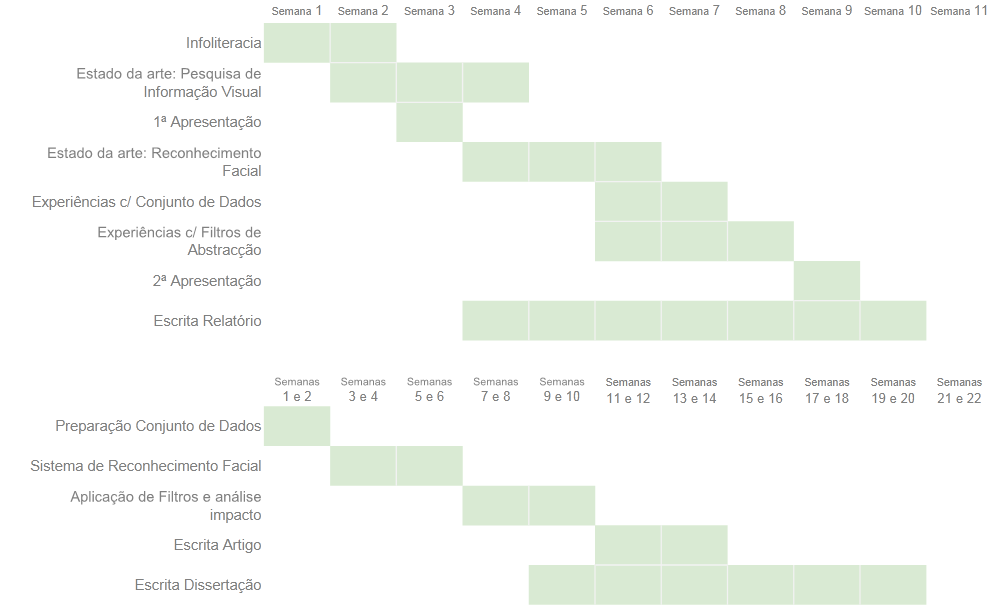
\includegraphics[width=0.9\textwidth]{GantSemSemanas}
    \caption{Plano de Trabalho 1º e 2º Semestres}	
    \label{fig:planotrabalho}
  \end{center}
\end{figure}

//Novo gant só com 2º semestre?

%Adicionalmente propõe-se também o desenvolvimento de um sistema de reconhecimento facial de personalidades que integre a abstração de imagens no processo de reconhecimento facial. Este sistema deverá ser capaz de detetar as faces presentes numa imagem e apresentar uma lista de possíveis entidades nela contidas.
